Real agents were located in Copenhagen, Denmark and cloud provider data center was based in city Council Bluffs, Iowa, United States. That positions them roughly 7500km apart from each other what might contribute to significant time delays.

24 hour latency test was conducted in order to gather more insight on expected latency between agents and the cloud. During the test ICMP package with 32 bytes of data was send every minute to the cloud broker endpoint and Round Trip Time(RTT) was measured. Results can be seen on diagram \ref{fig:ping}.

\begin{figure}[H]
    \centering
    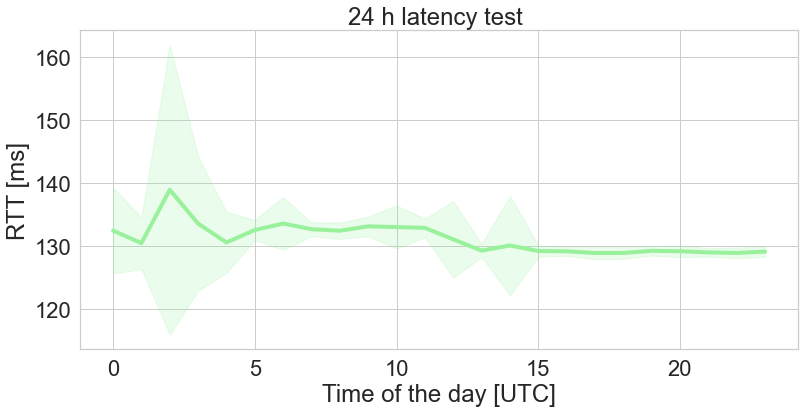
\includegraphics[width=0.8\textwidth]{pictures/ping.png}
    \caption{ RTT time }
    \label{fig:ping}
\end{figure}

During 24h test average RTT was around 131ms, min 126ms, max 236ms, std 6ms over whole test. Largest standard deviation can be seen between 1 and 4 AM UTC.